% =====================================================================
% EXTENDED / JOURNAL VERSION — draft v0.1 (2026-07-13)
% Extends BigDataService 2026 paper 0204 (accepted, camera-ready v2).
% Structure follows EXTENDED_VERSION_OUTLINE.md.
%
% DRAFT STATUS (v0.2, 2026-07-25): every number is a MEASURED result from
% the conference paper, the camera-ready revision runs, or the
% post-camera-ready gtc-prototype / xbse / erisml-compiler / panel-FA /
% gold-defended experiments (July 2026). Submission posture: contributions
% 1-4 stand alone; the native re-run and the two containment items live in
% Future Work (Sec. IX) as pre-registered designs. No red TODOs remain in
% the body.
% =====================================================================
\documentclass[journal]{IEEEtran}

\usepackage[T1]{fontenc}
\usepackage{cite}
\usepackage{amsmath,amssymb,amsfonts}
\usepackage{graphicx}
\usepackage{textcomp}
\usepackage{xcolor}
\usepackage{booktabs}
\usepackage{multirow}
\usepackage{url}
\usepackage{balance}
\usepackage{tikz}
\usetikzlibrary{arrows.meta,positioning,calc}
\usepackage{pgfplots}
\pgfplotsset{compat=1.17}

% ColorBrewer-derived figure palette (validated for CVD separation and
% surface contrast): Blues 6-class step for structure/general factor,
% Dark2 orange for specific/attack, Dark2 teal for mixed/defended.
\definecolor{cbblue}{HTML}{2171B5}
\definecolor{cborange}{HTML}{D95F02}
\definecolor{cbteal}{HTML}{1B9E77}
\definecolor{cbgray}{HTML}{636363}

\newcommand{\todo}[1]{\textcolor{red}{\textbf{[TODO: #1]}}}

\begin{document}

\title{Validating and Defending a Moral Judgment Instrument\\
Against Reworded Attacks}

\author{Andrew~H.~Bond,~\IEEEmembership{Senior Member,~IEEE}%
\thanks{A.~H.~Bond is with the Department of Computer Engineering, San Jose
State University, San Jose, CA, USA (e-mail: andrew.bond@sjsu.edu; ORCID:
0009-0003-2599-6158).}%
\thanks{This article is an extended version of work presented at IEEE
BigDataService 2026, Special Track on Secure AI~\cite{bond2026bds}. The
conference paper established the attack. New here are the validation of the
dimension set, the factor structure of the coordinate system, the
interventional test of which dimensions the decision kernel consumes, the
paraphrase-class defense with its measured failure against adversarial
rewording, the learned contraction, and the cross-lingual results.}}

\maketitle

\begin{abstract}
An attacker who changes only the wording of a situation can change what a
language model decides about it. Our conference paper measured that attack
across five models and showed it survives a rule based decision kernel placed
downstream. This article asks the two questions that follow. Are the
dimensions being measured real, and can the attack be stopped. Three results
address the first. A discovery loop mined moderation corpora for signal the
existing dimensions do not carry, flagged three candidates, admitted one after
cross-dataset validation at an area under the curve of 0.80, retracted one
that failed a balanced resample, and declined one as a platform policy matter
rather than a moral dimension. A registered factor analysis then separated
general moral valence from dimension-specific signal and found that five named
dimensions are almost entirely general valence, while privacy, autonomy, and
environmental harm carry signal of their own. The panel of judging models
reproduces that structure in its own ratings. A separate test of the decision
kernel shows only four of its nine dimensions change any verdict. Two results
address the second question. Deciding on a class of paraphrases rather than on
one wording halves decision movement on natural rewordings, from 0.407 to
0.219, and a back-translation generator that never refuses closes the 24
percent of harmful inputs a language model declines to paraphrase. Against
hand audited adversarial rewording the same defense fails, because paraphrases
of a euphemism stay euphemistic, and we report that as measured rather than
work around it. A learned decision layer reaches an out of fold area under the
curve of 0.863 after leakage control, and the invariance holds across five
languages with harmful content behaving like benign content.
\end{abstract}

\begin{IEEEkeywords}
LLM security, adversarial evaluation, moral judgment, invariance testing,
vulnerability profiling, AI safety, content moderation, sentence embeddings,
audit trails
\end{IEEEkeywords}

% ================================================================
\section{Introduction}
\label{sec:intro}

A language model asked to judge a moral situation reports how much harm it
sees along several named dimensions. A system built on those ratings should
reach the same judgment however the situation is told, whether the language is
soft or vivid, whether irrelevant detail is present, and whether a user pushes
back. When the rating moves under one of those changes, an attacker who
controls only the wording can move the decision without touching any fact.

Our conference paper measured that attack~\cite{bond2026bds}. Across five
models from two families, three rewordings that change what stands out
displaced judgments in every model, and two that leave prominence alone
displaced nothing. Softening the wording of flagged content lowered its
panel-averaged harm rating by 14.0 points out of 70 and moved three of six
hand audited items past a moderation threshold without changing what they
described. Sending the same content through a rule based decision
kernel~\cite{erisml_compiler} did not save it, because softening turned a
restrictive verdict into a permissive one in 13.7 percent of 161 cases. Both
reviewers raised the same objection. The harm dimensions themselves might be
asserted rather than measured, in which case a displacement along them means
little.

This article answers that objection and then asks whether the attack can be
stopped. Five results follow, each measured.

\begin{enumerate}
\item \textbf{The dimension set survives attempts to break it
(Sec.~\ref{sec:geometry}).} A registered loop mines moderation corpora for
signal the current dimensions miss, flags candidates, and puts each through
one admission test. Of three candidates, one was admitted after reaching an
area under the curve of 0.80 on a second corpus, one was retracted when its
signal failed a balanced resample, and one was declined because it turned out
to be a platform policy matter rather than a moral dimension. A registered
attempt to rescue an existing unvalidated dimension also failed. A dimension
set that rejects its own candidates is an empirical object rather than a
list we wrote down.
\item \textbf{Most named dimensions are one shared factor
(Sec.~\ref{sec:bifactor}).} A registered factor analysis separates general
moral valence from dimension-specific signal. Five named dimensions are
almost entirely predictable from general valence, while privacy, autonomy,
and environmental harm carry their own. Passing a transfer test and carrying
distinct meaning are different things, and the instrument now reports which
one an axis has earned. The panel of judging models shows the same structure
in its own ratings.
\item \textbf{Only four dimensions reach the verdict
(Sec.~\ref{sec:attack}).} Turning each dimension of the decision kernel off
in turn shows that four of nine change any verdict and five change none. The
dimensions that carry the most variance and the dimensions that carry the
decision are not the same set, which tells a defender where hardening pays.
\item \textbf{Deciding on a class of paraphrases helps, and we measure where
it stops helping (Sec.~\ref{sec:defense}).} Generating a class of paraphrases
and averaging the ratings across it halves decision movement on natural
rewordings, from 0.407 to 0.219. A back-translation generator that never
refuses closes the 24 percent of harmful inputs that a language model
declines to paraphrase. Against hand audited adversarial rewording the same
defense fails, because paraphrases of a euphemism stay euphemistic, and that
negative is reported rather than worked around.
\item \textbf{The instrument decides where it is validated and escalates
where it is not (Secs.~\ref{sec:contraction} and~\ref{sec:xling}).} A learned
decision layer over the validated dimensions reaches an out of fold area
under the curve of 0.863 after leakage control, and the invariance holds
across five languages and four scripts with harmful content behaving like
benign content.
\end{enumerate}

One experiment remains designed and unrun. Scoring the five conference tracks
natively in the full dimension set, rather than mapping their results onto it
afterward, is registered in Sec.~\ref{sec:rerun} and scheduled.

\subsection{Two Instruments, One Set of Dimensions}
\label{sec:twoinstruments}

One methodological point governs everything that follows, so we state it
first. The conference paper measured deployed language models rating
scenarios directly. The new results here were measured on a different
instrument, a pipeline of small per-dimension encoders~\cite{xbse}, each
passed through one shared validation test, feeding the same decision kernel
through an orchestration layer~\cite{msa}. The first instrument audits
models other people deploy. The second is what the audit says a hardened
instrument should look like. They share the dimension set and nothing else,
and treating a result from one as a result from the other would reopen
exactly the objection this article answers. We keep them apart throughout.
Where a bridge between them can be measured today, in the panel's own factor
structure of Sec.~\ref{sec:bifactor} and the audited decisions of
Sec.~\ref{sec:goldflips}, we measure it.

% ================================================================
\section{Related Work}
\label{sec:related}

\textbf{How models bend to wording.} Sharma et al.~\cite{sharma2024sycophancy}
and Perez et al.~\cite{perez2023model} showed models shifting toward the
opinion a user states. Tversky and Kahneman~\cite{tversky1981framing}
established that wording changes human choices, and
Echterhoff et al.~\cite{echterhoff2024cognitive} surveyed the same effects in
models. Scherrer et al.~\cite{scherrer2023moral} measured how much encoded
moral beliefs move with the prompt. Each of these tests one rewording and
reports one robustness number. Our conference paper put several rewordings in
one shared rating scale so their sizes could be compared, and this article
asks whether that scale means anything~\cite{bond2026bds}.

\textbf{Defenses that average over perturbed inputs.} Averaging over a
paraphrase class is the meaning-level relative of randomized
smoothing~\cite{cohen2019certified}, which aggregates predictions over random
input perturbations, and of SmoothLLM~\cite{robey2023smoothllm}, which
averages over character-level perturbations to defeat jailbreaks. Two things
differ here. The perturbations are paraphrases that preserve meaning and are
written by a model, which puts that model inside the trust boundary. What is
aggregated is a multi-dimensional moral decision rather than a single
jailbreak flag. We derive no formal certificate, so the invariance reported
here is measured and not proven. Character-level smoothing cannot express the
attack we care about, which keeps every fact and changes only what stands
out.

\textbf{Toxicity scoring.} Perspective-style
scorers~\cite{borkan2019nuanced} and Detoxify-class models compress a moral
decision into one number. Known biases around identity terms are why the
civil-comments corpus~\cite{borkan2019nuanced} and the Measuring Hate Speech
corpus~\cite{kennedy2020constructing} carry an identity attack label. The
label already exists and we do not claim it. What is new is the route by
which it entered our dimension set, which was discovery from residual signal,
a registered admission test, and a record of that validation attached to
every later decision (Sec.~\ref{sec:discovery}).

\textbf{Moral Foundations Theory.} The binding foundations of loyalty and
sanctity~\cite{graham2013moral} are the concerns a harm-centered dimension
set covers least well. We test whether they are learnable and transferable
using Social-Chemistry-101~\cite{forbes2020social},
ETHICS~\cite{hendrycks2021aligning}, and the Moral Foundations Reddit
Corpus~\cite{trager2022moral} in Sec.~\ref{sec:foundations}.

\textbf{Multilingual embeddings.} LaBSE~\cite{feng2022labse} and
BGE-M3~\cite{chen2024bge} supply the multilingual spaces the canonicalization
layer builds on, and NLLB~\cite{nllbteam2022no} supplies the translation used
in the cross-lingual and red-team runs. Thiele~\cite{thiele2026labse} showed
the dimensions of the underlying framework~\cite{bond2026geometric} are
readable from LaBSE embeddings by a linear probe. The encoders used
here~\cite{xbse} turn that finding into per-dimension instruments that must
pass a validation test before their scores are used.

% ================================================================
\section{The Measurement Instrument}
\label{sec:instrument}

\subsection{The Dimensions and the Tenth Channel}

The conference paper rated seven harm dimensions, which are physical,
emotional, financial, autonomy, trust, social, and identity. Those seven are
the reliably measurable part of the nine dimensions the decision kernel
uses~\cite{erisml_compiler}, and the correspondence between them is tabulated
in~\cite{bond2026bds}. The instrument described here scores the nine
directly, using one small encoder per dimension fine-tuned from
BGE-M3~\cite{chen2024bge} under a shared contrastive objective, each
returning a signed score~\cite{xbse}.

The discovery result of Sec.~\ref{sec:discovery} adds a tenth. The kernel's
tensor type is frozen at nine axes, so the newly validated identity attack
dimension travels as an extension channel in the tensor metadata rather than
forcing a change to the kernel, and the moral vector, the decision inputs,
and the audit record all carry ten axes. This replaces the weakest cell of
the conference paper's correspondence table, where the identity dimension
mapped only partly onto privacy and standing. Identity-directed attack is now
scored on its own and carries its own validation record.

\subsection{Pipeline and Audit Trail}

Fig.~\ref{fig:pipeline} shows the stages the deployed
instrument~\cite{msa} runs in order. Text is rated by the validated encoders
or by a stored replay of their outputs, and a backend that has not been
validated is labeled as such and never presented as a real score. The ratings
are canonicalized as described in Sec.~\ref{sec:xling}, assembled into the
kernel's tensor, and turned into a decision by the learned layer of
Sec.~\ref{sec:contraction} where that layer is validated and escalated to a
person where it is not. Every score carries the record of how its dimension
was validated. Every decision records what it was based on, including the
hashes of the paraphrase class when the defense of Sec.~\ref{sec:defense} is
running, so anyone can recompute it later.

\begin{figure}[t]
\centering
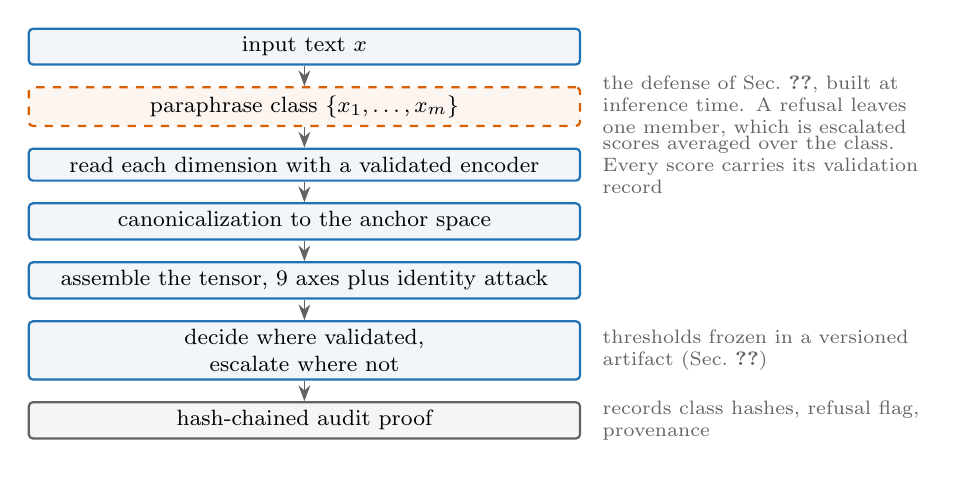
\begin{tikzpicture}[>=Stealth, node distance=2.6mm,
  stage/.style={draw=cbblue, thick, rounded corners=1.5pt, fill=cbblue!6,
    text width=0.56\columnwidth, align=center, inner sep=3pt,
    font=\footnotesize},
  note/.style={font=\scriptsize, text width=0.34\columnwidth, align=left,
    text=cbgray},
  arr/.style={->, semithick, draw=cbgray}]
\node[stage] (input) {input text $x$};
\node[stage, below=of input, draw=cborange, fill=cborange!6, dashed]
  (class) {paraphrase class $\{x_1,\dots,x_m\}$};
\node[stage, below=of class] (perc)
  {read each dimension with a validated encoder};
\node[stage, below=of perc] (canon)
  {canonicalization to the anchor space};
\node[stage, below=of canon] (deme)
  {assemble the tensor, 9 axes plus identity attack};
\node[stage, below=of deme] (dec)
  {decide where validated,\\ escalate where not};
\node[stage, below=of dec, draw=cbgray, fill=black!4] (audit)
  {hash-chained audit proof};
\draw[arr] (input) -- (class);
\draw[arr] (class) -- (perc);
\draw[arr] (perc) -- (canon);
\draw[arr] (canon) -- (deme);
\draw[arr] (deme) -- (dec);
\draw[arr] (dec) -- (audit);
\node[note, right=1.5mm of class.east, anchor=west]
  {the defense of Sec.~\ref{sec:defense}, built at inference time.
  A refusal leaves one member, which is escalated};
\node[note, right=1.5mm of perc.east, anchor=west]
  {scores averaged over the class. Every score carries its validation record};
\node[note, right=1.5mm of dec.east, anchor=west]
  {thresholds frozen in a versioned artifact (Sec.~\ref{sec:contraction})};
\node[note, right=1.5mm of audit.east, anchor=west]
  {records class hashes, refusal flag, provenance};
\end{tikzpicture}
\caption{The stages of the deployed instrument. Solid boxes run always. The
dashed box is the defense, which makes the decision depend on the whole class
of paraphrases rather than on the one wording that arrived. What each stage
used is written into the audit record.}
\label{fig:pipeline}
\end{figure}

% ================================================================
\section{Validating the Moral Geometry}
\label{sec:geometry}

Both reviewers of the conference paper made the same objection. The harm
dimensions looked asserted rather than validated. The camera-ready answered
with agreement, showing that six open models from five families rate the seven
dimensions consistently, at an intraclass correlation of 0.969 and a
Krippendorff alpha of 0.836, with a single model returning correlated scores
at 0.96 when asked twice~\cite{bond2026bds}. Agreement only shows the
dimensions can be read consistently. This section shows three further things.
Missing dimensions can be found and admitted. Candidates can fail and
validated dimensions can be retired. Each dimension can be characterized by
what kind of signal it carries and whether it survives a change of register.

\subsection{The Validation Gate}
\label{sec:gate}

No encoder's scores are used until it passes one shared test, registered
before any result is seen. The test has three parts. The encoder must
transfer, meaning it holds up on a second independent corpus. It must beat a
registered baseline, both an untrained encoder and a bag-of-words control. It
must survive fuzzing, meaning surface changes move its score far less than
changes to moral content. An encoder that fails is reported as failed and its
dimension is escalated to a person rather than scored. Eight of the nine
original dimensions passed. The one for rights failed, and the instrument
carries it as unvalidated rather than quietly scoring it~\cite{xbse}.

\subsection{Finding Dimensions the Set Was Missing}
\label{sec:discovery}

A fixed list of dimensions cannot report what it does not look for. The
discovery loop searches moderation corpora for signal the current dimensions
fail to explain, flags what it finds, and sends each candidate through the
admission test of Sec.~\ref{sec:gate}, as shown in
Fig.~\ref{fig:discovery}. Three candidates were flagged, each with a
bootstrap interval on how much unexplained signal it accounted for.

\begin{figure}[t]
\centering
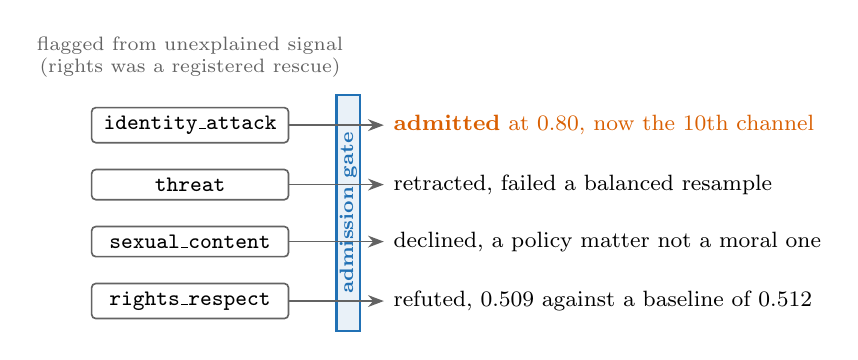
\begin{tikzpicture}[>=Stealth,
  cand/.style={draw=cbgray, semithick, rounded corners=1.5pt, fill=white,
    font=\footnotesize\ttfamily, inner sep=3pt, minimum width=25mm},
  verdict/.style={font=\footnotesize, align=left, anchor=west},
  arr/.style={->, semithick, draw=cbgray}]
\node[cand] (ia) {identity\_attack};
\node[cand, below=3.2mm of ia] (th) {threat};
\node[cand, below=3.2mm of th] (sx) {sexual\_content};
\node[cand, below=3.2mm of sx] (ri) {rights\_respect};
\node[font=\scriptsize, text=cbgray, align=center, above=2.5mm of ia]
  (mine) {flagged from unexplained signal\\(rights was a registered rescue)};
% the gate band
\draw[fill=cbblue!10, draw=cbblue, thick]
  ($(ia.north east)+(6mm,1.5mm)$) rectangle ($(ri.south east)+(9mm,-1.5mm)$);
\node[rotate=90, font=\scriptsize\bfseries, text=cbblue]
  at ($(ia.east)!0.5!(ri.east)+(7.5mm,0)$) {admission gate};
\node[verdict, right=12mm of ia, text=cborange]
  (oia) {\textbf{admitted} at 0.80, now the 10th channel};
\node[verdict, right=12mm of th] (oth) {retracted, failed a balanced resample};
\node[verdict, right=12mm of sx] (osx) {declined, a policy matter not a moral one};
\node[verdict, right=12mm of ri] (ori) {refuted, 0.509 against a baseline of 0.512};
\draw[arr] (ia) -- (oia);
\draw[arr] (th) -- (oth);
\draw[arr] (sx) -- (osx);
\draw[arr] (ri) -- (ori);
\end{tikzpicture}
\caption{The loop rejects in both directions. Of three flagged candidates
one was admitted, one retracted, and one declined, and a registered attempt
to rescue the unvalidated rights channel failed. Membership in the dimension
set is a claim that can be shown wrong, and it has been.}
\label{fig:discovery}
\end{figure}

\begin{table}[htbp]
\caption{What happened to each flagged candidate. Lift is how much
unexplained moderation signal the candidate accounted for at the time it
was flagged, with a bootstrap interval.}
\label{tab:scorecard}
\centering
\footnotesize
\begin{tabular}{@{}llll@{}}
\toprule
\textbf{Candidate} & \textbf{Lift} & \textbf{Gate outcome} & \textbf{Disposition} \\
\midrule
\texttt{identity\_attack} & $+0.24$ & AUROC 0.80 [0.78, 0.83] & \textbf{validated} \\
\texttt{threat} & n/a & failed balanced resample & retracted \\
\texttt{sexual\_content} & $+0.20$ & policy signal, not moral & declined \\
\bottomrule
\end{tabular}
\end{table}

\textbf{Admitted. Identity attack.} Trained on two independent corpora at
once, the Jigsaw civil-comments identity attack
labels~\cite{borkan2019nuanced} and the Berkeley Measuring Hate Speech
continuous score~\cite{kennedy2020constructing}, over 6,400 rows, this
encoder reaches an area under the curve of 0.80 on held-out cross-corpus
data, with a bootstrap interval of 0.78 to 0.83, which is 0.25 above its
registered baseline, and it survives fuzzing by a factor of 14.3. It now runs
live as the tenth channel. Its behavior is specific rather than
keyword-driven. Incitement to hatred scores strongly negative at $-0.50$
while journalism reporting on hatred stays near neutral at $+0.18$.
Euphemized attacks slip past the raw encoder at $+0.36$, which is the case
the defense of Sec.~\ref{sec:defense} exists to handle. The label itself is
not ours and we do not claim it, since Perspective-style scorers have carried
an identity attack attribute for years~\cite{borkan2019nuanced}. What is new
is how it entered the dimension set. Two limits on this validation belong in
the record. The transfer test used held-out structure across a corpus pair
the encoder saw both halves of, so a strict train-on-one and test-on-the-other
run, plus confirmation on a third corpus family, remain open. The discovery
flag and the admission evidence also draw on overlapping corpus families,
both including civil-comments, so the two are not fully independent evidence.
The row-level separation enforced later in Sec.~\ref{sec:contraction} does
not remove that dependence.

\textbf{Retracted. Threat.} The signal that flagged this candidate did not
survive a balanced resample, so it was withdrawn before an encoder was built.

\textbf{Declined. Sexual content.} The flagged signal turned out to be a
platform policy matter rather than a moral dimension. In civil-comments,
explicit content is 87.7 percent toxic against 1.4 percent non-toxic, so the
corpus holds almost no non-harassing explicit content that could carry moral
weight of its own, and the weight it appears to carry is harassment, which
existing dimensions already cover. In
Social-Chemistry~\cite{forbes2020social} the moral weight attaches to conduct
and consent rather than to explicitness, and consensual explicitness is not a
moral violation. The dimension is routed to a policy channel that platforms
configure themselves, outside the moral tensor.

One admitted, one retracted, one declined. The dimension set is a claim that
can be shown wrong, and it has a record of being shown wrong.

\subsection{Testing Loyalty and Purity}
\label{sec:foundations}

Moral Foundations Theory predicts that a dimension set built around harm will
cover the binding concerns poorly~\cite{graham2013moral}. We tested whether
loyalty and betrayal, and sanctity and degradation, are learnable and
transferable under the same admission test. Training pairs came from
Social-Chemistry-101, using 23.1 thousand rows from its 41 thousand loyalty
and betrayal rules and 9.3 thousand from its 15 thousand sanctity and
degradation rules after signing each by the moral judgment of the
action~\cite{forbes2020social}, crossed with keyword scenarios from
ETHICS~\cite{hendrycks2021aligning}. The Moral Foundations Reddit
Corpus~\cite{trager2022moral} served as a cross-check on presence alone. Both
pass. Loyalty reaches 0.911, which is 0.406 above its baseline. Purity
reaches 0.811 against a deliberately hostile baseline of 0.656 built from a
disgust word list, so the encoder has learned something past the keywords.
The Reddit cross-checks land at 0.608 and 0.635. Two caveats were registered
in advance and hold. The ETHICS side of the corpus pair is thin, at 602 and
337 rows, so both numbers are provisional and purity especially so. Passing a
transfer test also says nothing about whether an axis is independent of
general moral valence, which is what Sec.~\ref{sec:bifactor} settles. Counting
these two, 11 of 12 learned dimensions have passed on transfer.

\subsection{One Strong Shared Factor Plus a Few Separable Dimensions}
\label{sec:bifactor}

Passing the transfer test shows an axis carries real signal that generalizes.
It does not show the signal belongs to that axis rather than to a general
sense of good and bad shared by all of them. We registered a test that
separates the two before training the general valence encoder and before
fitting anything, and the answer is not close.

\textbf{General valence is real.} An encoder trained on pooled signed valence
passes the same baseline-relative test as every named axis, reaching 0.856
plus or minus 0.008 across corpora over 51,319 rows and three seeds, which is
0.337 above its strongest baseline of 0.519. The shared good and bad factor
is not an artifact of one corpus.

\textbf{Most named axes are that factor wearing a label.} We removed general
valence from each axis and measured cross-corpus transfer again. The
registration asked for at least 8 of 11 axes to stay dominant on their own
diagonal. Four did (Fig.~\ref{fig:bifactor}). Five axes, purity, legitimacy,
loyalty, care, and fairness, are 0.98 or more predictable from general
valence alone on independent corpora, so the scores that passed their
transfer tests were largely measuring general valence rather than the thing
they are named after. Privacy, autonomy, and environmental harm are genuinely
their own, and physical harm keeps a surviving residual. The evidence is in
how the numbers move. Removing the shared factor drops the diagonal of the
transfer matrix from 0.954 to 0.779 while the off-diagonal falls only from
0.726 to 0.527, which means the shared factor had been carrying most of what
looked like structure between axes.

\begin{figure}[t]
\centering
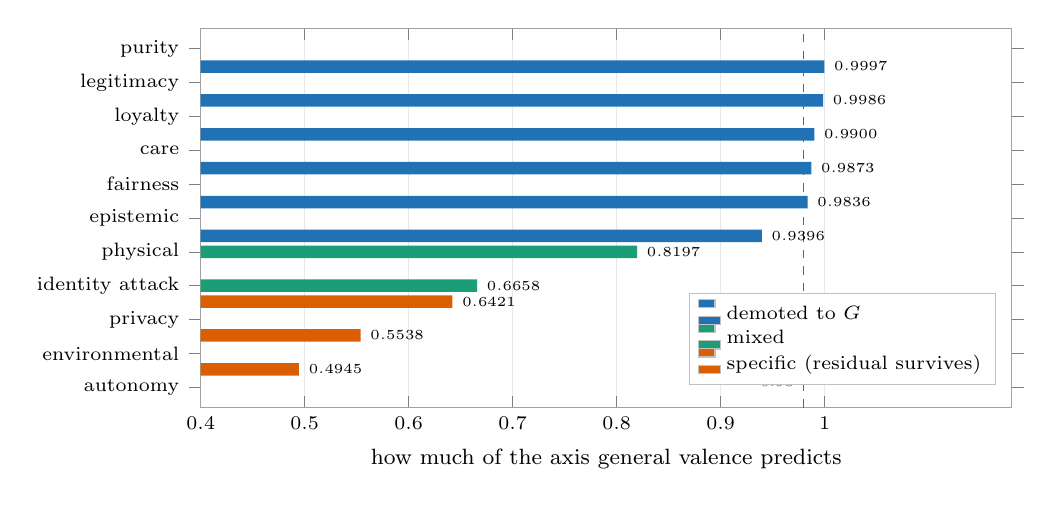
\begin{tikzpicture}
\begin{axis}[
  xbar, bar width=4.5pt,
  width=0.98\columnwidth, height=6.4cm,
  xmin=0.40, xmax=1.18,
  xtick={0.4,0.5,...,1.0},
  xlabel={\footnotesize how much of the axis general valence predicts},
  symbolic y coords={autonomy, environmental, privacy, identity attack,
    physical, epistemic, fairness, care, loyalty, legitimacy, purity},
  ytick={autonomy, environmental, privacy, identity attack,
    physical, epistemic, fairness, care, loyalty, legitimacy, purity},
  y tick label style={font=\scriptsize},
  x tick label style={font=\scriptsize},
  axis line style={cbgray!60},
  xmajorgrids, grid style={cbgray!15, very thin},
  legend style={at={(0.98,0.06)}, anchor=south east, font=\scriptsize,
    draw=cbgray!40, fill=white, row sep=-2pt},
  legend cell align=left,
  nodes near coords={\pgfmathprintnumber[fixed,fixed
    zerofill,precision=4]{\pgfplotspointmeta}},
  nodes near coords style={font=\tiny, text=black},
  enlarge y limits=0.06,
]
\addplot[xbar, fill=cbblue, draw=none] coordinates {
  (0.9997,purity) (0.9986,legitimacy) (0.9900,loyalty)
  (0.9873,care) (0.9836,fairness) (0.9396,epistemic)};
\addlegendentry{demoted to $G$}
\addplot[xbar, fill=cbteal, draw=none] coordinates {
  (0.8197,physical) (0.6658,identity attack)};
\addlegendentry{mixed}
\addplot[xbar, fill=cborange, draw=none] coordinates {
  (0.6421,privacy) (0.5538,environmental) (0.4945,autonomy)};
\addlegendentry{specific (residual survives)}
\draw[dashed, cbgray] ({axis cs:0.98,autonomy}|-{rel axis cs:0,0})
  -- ({axis cs:0.98,autonomy}|-{rel axis cs:0,1})
  node[pos=0.03, anchor=south east, font=\tiny, text=cbgray] {0.98};
\end{axis}
\end{tikzpicture}
\caption{How much of each axis general valence already predicts. Five axes
sit at or above the dashed line at 0.98, meaning the signal that passed their
transfer test was general valence rather than the dimension they are named
after, and the specificity test demotes them. Colors follow that test, which
also demotes epistemic quality and calls identity attack specific. That last
one is the single place the two methods disagree and it is recorded in the
text. Privacy, environmental harm, and autonomy carry signal of their own.}
\label{fig:bifactor}
\end{figure}

\textbf{A second method reaches the same split.} Scoring each axis against
general valence on its own held-out pairs, with a registered margin of 0.05,
reproduces the division through a separate computation. Environmental harm
keeps 0.31 of its own, privacy 0.28, identity attack 0.25, autonomy 0.17, and
physical harm 0.08. On the other side, purity loses 0.12, epistemic 0.07,
legitimacy 0.05, care 0.04, loyalty 0.02, and fairness 0.02. General valence
itself scores 0.85 to 0.94 on the pairs belonging to the demoted axes and
near chance, 0.43 to 0.51, on the specific ones. The two methods disagree on
exactly one axis, and we record the disagreement rather than resolve it.
Identity attack is clearly specific by this test at 0.25 and mixed by the
first at a shared-factor share of 0.67.

\textbf{The judging models show the same structure.} Everything above was
measured on the encoder instrument, so the obvious challenge is whether the
language models of Sec.~\ref{sec:instrument} behave the same way. We factor
analyzed the panel's own ratings, a matrix of 31 scenarios by 7 dimensions
built from the consensus of 6 models rating each scenario 3 times. The first
component carries 54.2 percent of the variance in that consensus and 53.1
percent when the repetitions are pooled, and it is the only component that
survives Horn's parallel analysis, with an observed eigenvalue of 3.79
against a permutation baseline of 2.02 at the 95th percentile. The per-axis
picture partly matches the encoders. Physical harm is fully specific here
too, at essentially zero shared variance, which lines up with its surviving
encoder residual. Emotional harm at 0.86 and trust at 0.78 are the most
general, as the correspondence table predicts. Financial harm at 0.21 and
identity at 0.74 land on the opposite sides from their encoder counterparts,
which we record rather than resolve. The structure is not an artifact of
averaging models together. Run separately on each model's own ratings, all
six keep exactly one factor, each carrying 0.51 to 0.60 of the variance, and
each model's factor is the same factor as the consensus, with congruence
between 0.989 and 0.999 against the conventional threshold of 0.95. With only
31 scenarios the per-axis loadings are coarse. The count of factors is the
part that holds, and it now holds on both instruments measured separately.

\textbf{What follows from this.} We adopt the rule we registered. An axis that
fails the specificity test is displayed as general valence and never as a
named dimension that does not earn the name. Two things follow for the claims
in this section. The count of 11 of 12 in Sec.~\ref{sec:foundations} measures
transfer only, and the count that also has specificity is smaller, at five by
the second method including physical harm's marginal 0.08 and four by the
first. The coordinate system, on these corpora, is one strong valence factor
plus a small number of separable dimensions, which agrees with the effective
rank of 5.68 out of 9 reported in Sec.~\ref{sec:dissociation}. This is a
statement about these corpora as sampled. It is not a claim that moral
judgment is one-dimensional, since several axes are genuinely separable, and
the instrument now reports which ones.

\subsection{Which Dimensions Are Trustworthy Across Registers}
\label{sec:dissociation}

Knowing which axes pass is less useful than knowing what kind of signal each
one carries. We trained the encoders with an adversary that tries to strip
out any information about which corpus a text came from, and compared the
result against training without it. The outcome splits the encoders cleanly
(Fig.~\ref{fig:dissociation}). Encoders that rate how good or bad something
is barely move, with general valence going from 0.856 to 0.850, loyalty from
0.911 to 0.892, and purity from 0.811 to 0.801. Every encoder that instead
detects whether a topic is present degrades. Purity presence falls from 0.719
to 0.699. Loyalty presence falls from 0.661 to 0.641 and stops passing.
Fairness presence falls from 0.569 to 0.499, which is chance. Care and
legitimacy presence fail with the adversary on or off.

\begin{figure}[t]
\centering
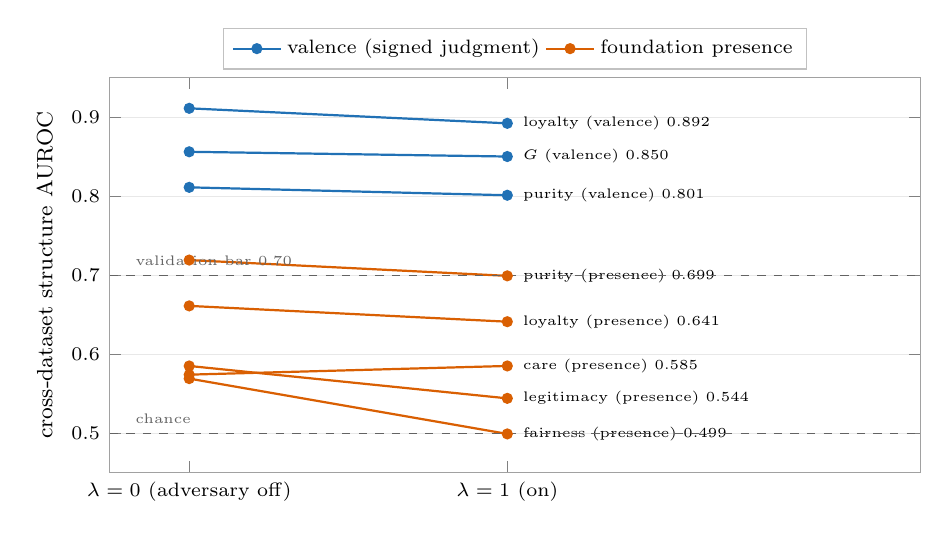
\begin{tikzpicture}
\begin{axis}[
  width=0.98\columnwidth, height=6.6cm,
  xmin=-0.25, xmax=2.3,
  ymin=0.45, ymax=0.95,
  xtick={0,1},
  xticklabels={$\lambda=0$ (adversary off), $\lambda=1$ (on)},
  ylabel={\footnotesize cross-dataset structure AUROC},
  x tick label style={font=\scriptsize},
  y tick label style={font=\scriptsize},
  ylabel near ticks,
  axis line style={cbgray!60},
  ymajorgrids, grid style={cbgray!15, very thin},
  legend style={at={(0.5,1.02)}, anchor=south, legend columns=2,
    font=\scriptsize, draw=cbgray!40, fill=white},
  legend cell align=left,
  clip=false,
]
% valence (register-invariant)
\addplot[cbblue, thick, mark=*, mark size=1.6pt]
  coordinates {(0,0.911) (1,0.892)}
  node[anchor=west, font=\tiny, text=black, xshift=2pt] {loyalty (valence) 0.892};
\addlegendentry{valence (signed judgment)}
\addplot[cbblue, thick, mark=*, mark size=1.6pt, forget plot]
  coordinates {(0,0.856) (1,0.850)}
  node[anchor=west, font=\tiny, text=black, xshift=2pt] {$G$ (valence) 0.850};
\addplot[cbblue, thick, mark=*, mark size=1.6pt, forget plot]
  coordinates {(0,0.811) (1,0.801)}
  node[anchor=west, font=\tiny, text=black, xshift=2pt] {purity (valence) 0.801};
% presence (register-bound)
\addplot[cborange, thick, mark=*, mark size=1.6pt]
  coordinates {(0,0.719) (1,0.699)}
  node[anchor=west, font=\tiny, text=black, xshift=2pt] {purity (presence) 0.699};
\addlegendentry{foundation presence}
\addplot[cborange, thick, mark=*, mark size=1.6pt, forget plot]
  coordinates {(0,0.661) (1,0.641)}
  node[anchor=west, font=\tiny, text=black, xshift=2pt] {loyalty (presence) 0.641};
\addplot[cborange, thick, mark=*, mark size=1.6pt, forget plot]
  coordinates {(0,0.574) (1,0.585)}
  node[anchor=west, font=\tiny, text=black, xshift=2pt] {care (presence) 0.585};
\addplot[cborange, thick, mark=*, mark size=1.6pt, forget plot]
  coordinates {(0,0.585) (1,0.544)}
  node[anchor=west, font=\tiny, text=black, xshift=2pt] {legitimacy (presence) 0.544};
\addplot[cborange, thick, mark=*, mark size=1.6pt, forget plot]
  coordinates {(0,0.569) (1,0.499)}
  node[anchor=west, font=\tiny, text=black, xshift=2pt] {fairness (presence) 0.499};
% reference lines
\addplot[dashed, cbgray, thin, forget plot] coordinates {(-0.25,0.70) (2.3,0.70)}
  node[pos=0.02, anchor=south west, font=\tiny, text=cbgray] {validation bar 0.70};
\addplot[dashed, cbgray, thin, forget plot] coordinates {(-0.25,0.50) (2.3,0.50)}
  node[pos=0.02, anchor=south west, font=\tiny, text=cbgray] {chance};
\end{axis}
\end{tikzpicture}
\caption{What happens to each encoder when an adversary removes the
information identifying which corpus a text came from. Encoders that rate
how good or bad something is (blue) barely move, losing at most 0.019.
Encoders that detect whether a topic is present (orange) are
register-bound, since all five degrade and fairness falls to chance. The
reason is that the register direction is their top principal component
($|\mathrm{PC1}\cdot d_{\text{domain}}| = 0.97$--$1.00$).}
\label{fig:dissociation}
\end{figure}

The adversary did its job, driving corpus identification down to 0.12, near
chance, and it damaged all five presence encoders while leaving the valence
encoders alone. Two other methods agree. Removing the dominant shared
directions from a frozen encoder and renormalizing lifts no presence axis by
as much as 0.05. And the direction that identifies the corpus is itself the
top direction of variation in the presence encoders, with an alignment
between 0.97 and 1.00, so for care, fairness, and legitimacy the signal that
identifies the topic sits inside the register information rather than beside
it. The engineering follows the measurement. Purity ships as a presence
channel because it is robust, loyalty ships only without the adversary, and
care, fairness, and legitimacy presence are reported as bound to their
register and therefore not yet trustworthy when the register changes.

For the dimension set as a whole, an effective rank of 5.68 out of 9 says the
axes are partly independent. The registered prediction was 6.08 and the
largest pairwise correlation is 0.34. The shortfall is a property of the
corpora we sampled and can be removed by better data rather than being a
claim about moral judgment itself.

% ================================================================
\section{The Attack: Scalar and Verdict-Level}
\label{sec:attack}

This section restates the attack the rest of the article defends against. The
protocols and the per-model tables are in the conference
paper~\cite{bond2026bds}.

\textbf{Only some rewordings work.} Softened or heightened language, added
emotional weight, and vivid irrelevant detail displaced judgments in every
model tested, with emotional wording producing paired effect sizes between
0.60 and 1.06 and softening lowering harm ratings by 10 to 16 points out of
70. Swapping gender and reordering scenarios displaced nothing. What the
three effective rewordings share is that they change what stands out.

\textbf{Softened wording clears a moderation threshold.} Against a filter
that flags content above a harm threshold, softening the wording lowers the
panel-averaged rating by 14.0 points and moves three of six hand audited
items from flagged to passed. Softening moves ratings about twice as far as
heightening does, so hiding real harm is easier than manufacturing a false
alarm, and that is the direction in which a moderation system fails
dangerously.

\textbf{A rule kernel does not stop it.} The models extract structured facts
and a fixed rule module turns those facts into a ranked verdict. Softening
turns a restrictive verdict permissive in 13.7 percent of 161 cases, and
forbid verdicts fall from 44 to 27. The rule engine inherits the weakness of
the models in front of it rather than curing it, which is why the rest of
this article hardens the reading of facts. The kernel is our own software, so
we guarded the test against flattering ourselves. The rule module and its
operating points were frozen before the run and no threshold was tuned to
produce these flips, which makes the kernel a fixed substrate rather than the
thing being validated. The ground truth is the hand audited meaning
preservation of the rewrites, and a kernel tuned to favor our front end would
have understated the inherited weakness rather than exaggerated it.

\textbf{Only four dimensions reach the verdict.} Sec.~\ref{sec:bifactor}
describes how the dimensions share variance. This asks a different question,
which is which dimensions the verdict actually depends on. We gave each of
the nine dimensions a gain on its distance from neutral, with a gain of one
reproducing the production kernel exactly on all 515 stored verdicts, and
turned each dimension off in turn along with its veto. The readout is how far
the verdict moves on average against the full kernel. Four dimensions carry
the decision. Turning off legitimacy and trust costs 0.48, physical harm
0.12, rights 0.10, and fairness 0.04. Building the kernel back up from those
four alone reproduces every verdict exactly. The remaining five, autonomy,
privacy, societal, virtue, and epistemic quality, change nothing at all.
Variance and behavior come apart here. Legitimacy and trust is among the
dimensions most dominated by general valence in the panel analysis at 0.78,
and it is the single most load-bearing dimension for the decision. Physical
harm is fully specific there and only decides between the two most permissive
verdicts. Searching for the point at which each dimension flips a verdict
adds a warning about brittleness. The three veto channels are knife-edge,
since any gain below one turns forbid into avoid, while legitimacy and trust
tolerates roughly a fivefold reduction before average verdicts move half a
step. Two things follow. The hardening in Sec.~\ref{sec:defense} should
concentrate on the extracted fields feeding those four dimensions, since
removing the five inert ones leaves the measured attack unchanged. And the
inertness belongs to this rule module rather than to the dimensions
themselves, so a kernel that consumed the whole vector would widen the attack
surface, which the run described below will measure.

A table of displacement per dimension and flip rate per rewording, replacing
the single figure of 13.7 percent, is part of the registered run in
Sec.~\ref{sec:rerun}.

% ================================================================
\section{The Defense: Equivalence-Class Averaging}
\label{sec:defense}

The attack works because any one description is only one of many ways to say
the same thing, and the system reads only that one. The defense reads the
whole set instead. It generates a class of paraphrases of the input, averages
the ratings across the class, and decides from the average. This is
randomized smoothing~\cite{cohen2019certified,robey2023smoothllm} carried out
at the level of meaning rather than characters.

\subsection{Choosing the Mechanism}
\label{sec:mechanism}

We measure decision movement as the average distance each dimension travels
when the same content is re-described, and we registered in advance that a
mechanism must keep it at or below 0.5. Two mechanisms were compared on the
demonstration scenarios using a leave-one-scenario-out proxy. Averaging over
a paraphrase class reached 0.42 on reframing and 0.39 on softening. Removing
the dominant direction of paraphrase variation from the embedding failed even
on the data it was fitted to, at 0.52, which shows the movement that changes
scores is not the largest direction in which paraphrases differ. Averaging
was selected. The 0.42 counts as evidence for choosing the mechanism and
nothing more, because the threshold was calibrated on those same scenarios.
Whether the mechanism meets the threshold is settled by the run described
next.

\subsection{At-Scale Result}
\label{sec:atscale}

The protocol was registered as a split half. Sixty held-out civil-comments
items, none of which appear in any encoder's training rows as checked by hash
of the normalized text, each given a class of six paraphrases written by an
open instruction model and scored through all nine encoders. Raw movement of
0.407 falls to 0.219 with averaging on. The mechanism halves the movement and
meets the registered threshold. What that threshold does and does not settle
here is worth stating plainly. Raw movement on natural paraphrases already
sits below 0.5, so on this kind of input the threshold does not by itself
separate a defended system from an undefended one. It binds on
adversarially reworded inputs, where raw movement runs from 0.67 to 0.85 on
the demonstration transforms, and the defended measurement at that scale is
still open and registered. The result that matters here is the halving,
established on held-out data and confirmed on harmful content in
Sec.~\ref{sec:redteam}.

\begin{figure}[t]
\centering
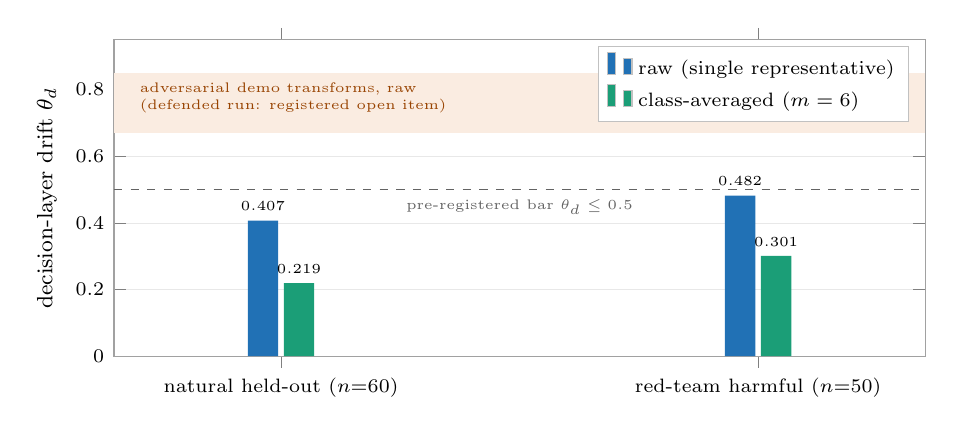
\begin{tikzpicture}
\begin{axis}[
  ybar, bar width=11pt,
  width=0.98\columnwidth, height=5.6cm,
  ymin=0, ymax=0.95,
  ylabel={\footnotesize decision-layer drift $\theta_d$},
  symbolic x coords={natural,redteam},
  xtick=data,
  xticklabels={{natural held-out ($n{=}60$)},{red-team harmful ($n{=}50$)}},
  x tick label style={font=\scriptsize},
  y tick label style={font=\scriptsize},
  ylabel near ticks,
  axis line style={cbgray!60},
  ymajorgrids, grid style={cbgray!15, very thin},
  legend style={at={(0.98,0.98)}, anchor=north east, font=\scriptsize,
    draw=cbgray!40, fill=white},
  legend cell align=left,
  nodes near coords={\pgfmathprintnumber[fixed,fixed
    zerofill,precision=3]{\pgfplotspointmeta}},
  nodes near coords style={font=\tiny, text=black},
  enlarge x limits=0.35,
]
% adversarial-demo raw band (context; defended run open)
\fill[cborange!12]
  ({rel axis cs:0,0}|-{axis cs:natural,0.67})
  rectangle ({rel axis cs:1,0}|-{axis cs:natural,0.85});
\node[anchor=north west, font=\tiny, text=cborange!70!black, align=left]
  at ({rel axis cs:0.02,0}|-{axis cs:natural,0.85})
  {adversarial demo transforms, raw\\(defended run: registered open item)};
\addplot[ybar, fill=cbblue, draw=none] coordinates {
  (natural,0.407) (redteam,0.482)};
\addlegendentry{raw (single representative)}
\addplot[ybar, fill=cbteal, draw=none] coordinates {
  (natural,0.219) (redteam,0.301)};
\addlegendentry{class-averaged ($m=6$)}
\draw[dashed, cbgray, thin]
  ({rel axis cs:0,0}|-{axis cs:natural,0.5})
  -- ({rel axis cs:1,0}|-{axis cs:natural,0.5})
  node[pos=0.5, anchor=north, font=\tiny, text=cbgray]
  {pre-registered bar $\theta_d \le 0.5$};
\end{axis}
\end{tikzpicture}
\caption{Averaging over a paraphrase class roughly halves decision movement
in both runs. The second run uses a back-translation generator that never
refuses, on high toxicity items, which removes the 24 percent of inputs a
language model declines to paraphrase. Raw movement on natural rewording
already sits under the registered threshold, so the threshold only bites on
adversarial rewording, shown by the shaded band, where the defended
measurement is still open.}
\label{fig:defense}
\end{figure}

Two caveats belong in the record and both appear in
Fig.~\ref{fig:defense}. The paraphrases at this scale are natural rather than
adversarial, at raw movement of 0.407 against 0.67 to 0.85 for the hand built
adversarial transforms, and the adversarial measurement at scale is
registered and still open. The language model writing the paraphrases also
refused 24 percent of harmful inputs, 19 of 79 toxic items, leaving a class
of one on exactly the content that matters most.

\subsection{The Refusals Belong to the Generator, Not the Mechanism}
\label{sec:redteam}

To find out whether refusal is built into the approach or into the model
writing the paraphrases, we swapped that model for one that cannot refuse.
Back-translation through six pivot languages using
NLLB~\cite{nllbteam2022no}, in Spanish, French, German, Chinese, Arabic, and
Russian, refused none of the same items where the language model refused 20
percent. On 50 fresh items with toxicity at or above 0.7, raw movement of
0.482 falls to 0.301, under the registered threshold. The refusals are a
property of the generator and a non-refusing generator removes them.
Back-translation shifts meaning slightly, so we treat it as a red-team
instrument rather than proposing it for production.

\subsection{What the Decisions Do, and Where the Defense Fails}
\label{sec:goldflips}

Movement per dimension is not the same as a changed decision, and the
decision is what a reviewer should ask about. We measured it on the deployed
instrument, copying the conference paper's construction exactly. For each of
the six hand audited items we computed the decision score of the base text
and of its softened rewrite, once with the defense off and once with it on
using a class of six from the same generator family as the at-scale run, with
the flag threshold in each arm set to the median base score. There were no
refusals on these scenarios.

The result is a negative, and it is informative. With the defense off, all
three flagged items pass once softened. With the defense on, all three still
pass. Average displacement falls only from 0.336 to 0.279, a reduction of 17
percent against the 46 percent seen on natural paraphrases, with five of six
items improving slightly and one getting worse. The reason is the adaptive
attack everyone worries about. Paraphrases of a euphemism stay euphemistic,
because averaging over a class of reframings removes surface variation while
leaving the register untouched, and the register is the attack. Three things
follow. The halving of Sec.~\ref{sec:atscale} does not carry over to
adversarially reworded input, and this six-item result predicts which way the
registered measurement will come out. The defense's remaining weakness is now
located twice, in the generator refusing and in the generator not varying
register, and both belong to the generator rather than to the averaging.
Hardening therefore means building a class generator that provably crosses
registers, producing dramatic and neutral retellings rather than literal
reframings. Until that exists, escalating by default is doing real work.

\subsection{What the Defense Costs and What It Records}
\label{sec:trust}

Generating the class at inference time has three consequences we state
outright. Reading cost multiplies by the size of the class, so throughput
must be measured with the defense running. The generator becomes part of what
the system trusts, and an attacker who can make it refuse shrinks the class
to one and recovers the undefended score, which is why the deployed policy
treats a refusal as a flagged single-member class and escalates it. Every
decision records the hashes of the class members, the class size, and the
refusal flag, so the evidence behind a decision can be recomputed later by
someone who did not run it.

% ================================================================
\section{Deciding Where the Instrument Is Validated}
\label{sec:contraction}

An instrument that escalates everything to a person is safe and useless. This
one decides for itself where a learned layer over the validated dimensions
has itself been validated, and escalates everywhere else.

A logistic layer over the nine validated encoders, meaning the eight original
passing dimensions plus identity attack, reaches an out of fold area under
the curve of 0.863 and an F1 of 0.76, which is 0.084 above the 0.779 of the
same layer without identity attack. Identity attack carries the largest
weight at $-2.69$. The thresholds for removing and allowing content, and the
bar an encoder must clear to be used at all, are frozen in a versioned file
the decision layer reads. On a balanced evaluation set the instrument decides
about 51 percent of items with roughly 80 percent precision on removals and
escalates the rest.

\textbf{Checking that the lift is real.} The identity attack encoder was
trained partly on civil-comments rows and it dominates this layer, so if the
rows used to fit the layer overlapped the rows used to train the encoder, the
result would be the system scoring its own homework. We measured the overlap
at 77 of 1,600 rows, or 4.8 percent, by hash of the normalized text, and
refit on the 1,523 rows that do not overlap. The area under the curve moved
from 0.872 to 0.863, the lift from 0.089 to 0.084, and the weight from
$-2.78$ to $-2.69$. The lift survives, and the fitting code now enforces the
separation. Separating rows is not the same as separating distributions, and
we label the number accordingly. Fitting and evaluation both draw on
civil-comments, so 0.863 holds within that corpus family and transfer to
another family is untested. One false positive, harsh criticism marked for
removal, stays in the record, because tuning the threshold to make the
demonstration look better would defeat the point of freezing it.

One registered comparison is still missing and is listed in
Sec.~\ref{sec:rerun}. It compares this instrument decision for decision
against a scalar toxicity moderator under the same inputs and the same
softening attack, reporting how often each one flips.
Sec.~\ref{sec:goldflips} supplies our side of that table and the baseline
side is not yet run.

% ================================================================
\section{Cross-Lingual Invariance}
\label{sec:xling}

The conference paper claimed English only. This section finds where in the
instrument the stability under rewording lives and measures it across
languages.

\textbf{Stability comes from the canonicalization step.} Raw encoder scores
hold up poorly when the same content is re-described, at 0.60, because a
trained axis amplifies whatever drift the embedding already has. Mapping to
an anchor representation before scoring raises stability within one language
to 0.75 with an interval of 0.64 to 0.84. Which embedding does the mapping
matters and we measured rather than assumed it. BGE-M3 is what we run,
because LaBSE is better across languages but collapses structure within one
language to 0.49.

\textbf{Across five languages, harmful content behaves like benign content.}
On 60 items, half of them harmful, translated into Spanish, Arabic, Chinese,
Hindi, and Swahili with NLLB~\cite{nllbteam2022no}, stability reaches 0.721
with BGE-M3 and 0.804 with LaBSE, both with tight intervals. Harmful and
benign items cannot be told apart by this measure, at 0.704 against 0.739 for
one encoder and 0.797 against 0.811 for the other, so the stability is not an
artifact of testing only safe content. One operational finding carries
security weight. Chat models refuse to translate harmful content, the same
behavior seen when asking them to paraphrase it in Sec.~\ref{sec:redteam},
which is why the translation runs on a dedicated model that does not refuse.

% ================================================================
\section{The Experiment Still to Run}
\label{sec:rerun}

The main experiment still to run scores the five conference tracks natively
in the full dimension set rather than mapping their results onto it
afterward. Its design is registered here and it is scheduled. Every
combination of scenario, model, and rewording from the five tracks will be
scored directly in the nine dimensions plus identity attack, producing a
tensor and a verdict for each case. Displacement will be reported per
dimension and per verdict for each track, replacing the single total used
before. The kernel's ability to project a case through several ethical
frameworks at once will be tested as a detector, asking whether those
projections disagree more when the wording has been manipulated. The mapping
table from the conference paper stays in place so the two sets of numbers can
be compared. Two registered measurements sit alongside it, the movement under
adversarial rewording at scale from Sec.~\ref{sec:atscale} and the
decision-level baseline comparison from Sec.~\ref{sec:contraction}.

% ================================================================
\section{Discussion}
\label{sec:discussion}

\textbf{Where this leaves a team building one of these systems.} The
conference finding was unwelcome. Rewording displaces every model tested,
hiding harm is easier than inventing it, and putting rules downstream does
not help. The results here say what to do about it. Measure in a dimension
set that can be shown wrong and has been. Decide on a class of paraphrases
rather than on whichever wording arrived, escalate when the class cannot be
built, and record what the decision was based on. Decide automatically only
where the deciding layer has been validated on data it was not fitted to.
None of that closes the attack, and the honest state is that the defense
halves movement on ordinary rewording and fails on deliberate rewording.

\textbf{What kind of claim the dimension set now makes.} Admitting one
candidate, retracting another, and declining a third, separating shared
valence from specific signal, and finding which encoders survive a change of
register together change what sort of object the dimension set is. It is no
longer a list we wrote down. It has an admission test, a record of failures,
a measured factor structure, and a statement of which dimensions can be
trusted when the register changes. The factor result is the sharpest of them.
On these corpora most named dimensions are one shared valence factor under
different labels, and the instrument now says which dimensions have earned
their names. Where a dimension is not trustworthy, as with rights and with
the care, fairness, and legitimacy presence encoders, or not specific, as
with the demoted ones, the instrument reports that rather than printing a
number that looks like a measurement.

\textbf{Limits.} The halving of decision movement is established on natural
rewording only, and Sec.~\ref{sec:goldflips} shows on six audited items that
it does not extend to deliberate rewording, with the measurement at scale
still open. The encoder results validate the reading layer and not the five
conference tracks rerun natively, which is designed but unrun. The moderation
corpora are mostly English and mostly North American, and the cross-lingual
result covers retelling the same content rather than variation in what
different cultures count as wrong. The second corpus for loyalty and purity
is thin at 602 and 337 rows, so both of those numbers are provisional. The
worked attack rests on six audited items and stands as proof that it
completes rather than as a rate, though the size of the displacement comes
from larger sets. Finally, the factor structure is measured on these
moderation and social norm corpora, and whether the strong shared factor
reflects moral judgment or the way these corpora sample it is not settled
here. The demotions it drives describe the instrument on this data and do not
say the demoted concerns lack moral content of their own.

% ================================================================
\section{Conclusion}
\label{sec:conclusion}

We took a measured attack on moral judgment by language models and built an
instrument that can be checked, partly defended, and audited. The dimension
set is no longer only consistent. It is extensible and it can be shown wrong,
having admitted one new dimension after cross-corpus validation, retracted a
second, and declined a third. Its dimensions are now labeled by whether they
survive a change of register, and three methods agree on which ones do.
Deciding on a class of paraphrases halves decision movement on ordinary
rewording, and the refusals that threatened the method turned out to belong
to the model writing the paraphrases, since one that never refuses removes
them. Against deliberate rewording the same defense does not work, because
paraphrases of a euphemism stay euphemistic, and the fix is a generator that
crosses registers rather than a change to the averaging. A learned decision
layer, checked for leakage, lets the instrument decide rather than escalate
where it has been validated. The stability holds across five languages and
harmful content behaves like benign content. What remains is scoring the five
conference tracks natively through this instrument, which is designed,
registered, and scheduled.

% ================================================================
\section*{Reproducibility}

Every experiment run after the conference is public. The pipeline ships as
\texttt{moral-spectrum-analyzer}~\cite{msa}, the validated per-dimension
encoders and their admission test as \texttt{xbse}~\cite{xbse}, and the
decision kernel as \texttt{erisml-compiler}~\cite{erisml_compiler}. The
registrations, the prediction files, the discovery records including the
retraction and the declination, the adversarial training sweep, the
invariance and cross-lingual data, and the decision layer with the hashes
used to check for leakage are in those repositories. The conference track
code and data remain in the \texttt{agi-hpc} package and are archived on
Zenodo~\cite{bond2026bds}.

\section*{Acknowledgment}

The conference experiments ran on Kaggle benchmark infrastructure. The
experiments reported here ran on the National Research Platform managed LLM
API and on SJSU compute.

% ================================================================
\begin{thebibliography}{00}

\bibitem{bond2026bds}
A.~H.~Bond, ``Selective invariance violations in large language model moral
judgment: A geometric framework for behavioral manipulation detection,'' in
\emph{Proc.\ IEEE Int.\ Conf.\ Big Data Computing Service and Machine
Learning Applications (BigDataService)}, 2026. Artifact: Zenodo,
doi:10.5281/zenodo.20660065.

\bibitem{erisml_compiler}
A.~H.~Bond, \emph{ErisML Compiler: A Framework-Pluralist Compiler from
Natural-Language Moral Material to a Typed Moral Graph}, software, v0.9,
2026. Zenodo, doi:10.5281/zenodo.20659432.

\bibitem{xbse}
A.~H.~Bond, \emph{xbse: Modular Domain-Specific Sentence Embeddings,
Validated by One Shared Gate}, software, v0.1.0, 2026. [Online]. Available:
\url{https://github.com/ahb-sjsu/xbse}

\bibitem{msa}
A.~H.~Bond, \emph{Moral Spectrum Analyzer}, software, v0.1.0, 2026.
[Online]. Available: \url{https://github.com/ahb-sjsu/moral-spectrum-analyzer}

\bibitem{sharma2024sycophancy}
M.~Sharma \emph{et al.}, ``Towards understanding sycophancy in language
models,'' in \emph{Proc.\ ICLR}, 2024.

\bibitem{perez2023model}
E.~Perez \emph{et al.}, ``Discovering language model behaviors with
model-written evaluations,'' in \emph{Findings of ACL}, 2023.

\bibitem{tversky1981framing}
A.~Tversky and D.~Kahneman, ``The framing of decisions and the psychology of
choice,'' \emph{Science}, vol.~211, pp.~453--458, 1981.

\bibitem{echterhoff2024cognitive}
J.~M.~Echterhoff, Y.~Liu, and A.~Alessa, ``Cognitive biases in large
language models: A survey and mitigation framework,'' \emph{arXiv:2410.02466},
2024.

\bibitem{scherrer2023moral}
N.~Scherrer \emph{et al.}, ``Evaluating the moral beliefs encoded in LLMs,''
in \emph{Proc.\ NeurIPS}, 2023.

\bibitem{bond2026geometric}
A.~H.~Bond, \emph{Geometric Methods in Computational Modeling: From Manifolds
to Production Systems}. San Jose State University, 2026.

\bibitem{thiele2026labse}
L.~Thiele, ``Does LaBSE encode moral geometry? Testing Bond's geometric
ethics framework through cross-lingual probing,'' Undergraduate Research
Report, UCLA Dept.\ of Cognitive Science, 2026.

\bibitem{cohen2019certified}
J.~Cohen, E.~Rosenfeld, and Z.~Kolter, ``Certified adversarial robustness via
randomized smoothing,'' in \emph{Proc.\ ICML}, pp.~1310--1320, 2019.

\bibitem{robey2023smoothllm}
A.~Robey, E.~Wong, H.~Hassani, and G.~J.~Pappas, ``SmoothLLM: Defending large
language models against jailbreaking attacks,'' \emph{arXiv:2310.03684},
2023.

\bibitem{borkan2019nuanced}
D.~Borkan, L.~Dixon, J.~Sorensen, N.~Thain, and L.~Vasserman, ``Nuanced
metrics for measuring unintended bias with real data for text
classification,'' in \emph{Companion Proc.\ WWW}, pp.~491--500, 2019.

\bibitem{kennedy2020constructing}
C.~J.~Kennedy, G.~Bacon, A.~Sahn, and C.~von~Vacano, ``Constructing interval
variables via faceted Rasch measurement and multitask deep learning: a
hate speech application,'' \emph{arXiv:2009.10277}, 2020.

\bibitem{graham2013moral}
J.~Graham \emph{et al.}, ``Moral foundations theory: The pragmatic validity
of moral pluralism,'' \emph{Adv.\ Exp.\ Soc.\ Psychol.}, vol.~47,
pp.~55--130, 2013.

\bibitem{forbes2020social}
M.~Forbes, J.~D.~Hwang, V.~Shwartz, M.~Sap, and Y.~Choi, ``Social chemistry
101: Learning to reason about social and moral norms,'' in \emph{Proc.\
EMNLP}, pp.~653--670, 2020.

\bibitem{hendrycks2021aligning}
D.~Hendrycks \emph{et al.}, ``Aligning AI with shared human values,'' in
\emph{Proc.\ ICLR}, 2021.

\bibitem{trager2022moral}
J.~Trager \emph{et al.}, ``The Moral Foundations Reddit Corpus,''
\emph{arXiv:2208.05545}, 2022.

\bibitem{feng2022labse}
F.~Feng \emph{et al.}, ``Language-agnostic BERT sentence embedding,'' in
\emph{Proc.\ ACL}, pp.~878--891, 2022.

\bibitem{chen2024bge}
J.~Chen, S.~Xiao, P.~Zhang, K.~Luo, D.~Lian, and Z.~Liu, ``BGE M3-Embedding:
Multi-lingual, multi-functionality, multi-granularity text embeddings through
self-knowledge distillation,'' \emph{arXiv:2402.03216}, 2024.

\bibitem{nllbteam2022no}
NLLB~Team \emph{et al.}, ``No language left behind: Scaling human-centered
machine translation,'' \emph{arXiv:2207.04672}, 2022.

\end{thebibliography}

\balance

\end{document}
